\documentclass[a4paper]{article}  

\usepackage{mathtools}
\usepackage{amsthm}
\usepackage{amssymb}
\usepackage{tikz}
\usepackage{algpseudocode}

\title{CS270 Homework 1}
\author{Valkyrie Savage}

\begin{document}
\maketitle

\begin{enumerate}
\item Routing and Fractional Flow
	\begin{enumerate}
	\item Following is a simple example of a graph in which the maximum congestion in optimal solutions to the path routing problem and the fractional flow problem differ, with the solution to the \textbf{path routing} on the left and the solution to the \textbf{fractional flow} on the right.
		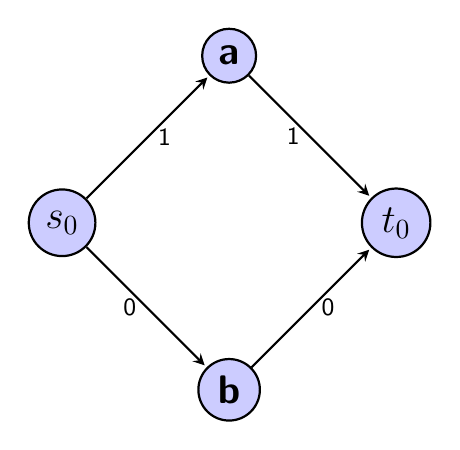
\begin{tikzpicture}[->,>=stealth,shorten >=1pt,auto,node distance=3cm,
 		thick,main node/.style={circle,fill=blue!20,draw,font=\sffamily\Large\bfseries}]

  		\node[main node] (B) {a};
  		\node[main node] (A) [below left of=B] {$s_0$};
  		\node[main node] (C) [below right of=A] {b};
  		\node[main node] (D) [below right of=B] {$t_0$};

  		\path[every node/.style={font=\sffamily\small}]
    		(B) edge node [left] {1} (D)
    		(A) edge node [right] {1} (B)
        		edge node [left]  {0} (C)
    		(C) edge node [right] {0} (D);
		\end{tikzpicture}
		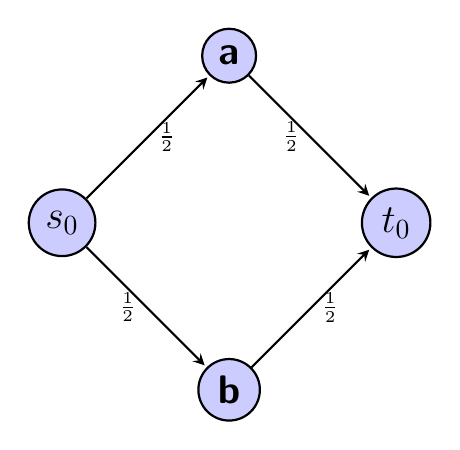
\begin{tikzpicture}[->,>=stealth,shorten >=1pt,auto,node distance=3cm,
 		thick,main node/.style={circle,fill=blue!20,draw,font=\sffamily\Large\bfseries}]

  		\node[main node] (B) {a};
  		\node[main node] (A) [below left of=B] {$s_0$};
  		\node[main node] (C) [below right of=A] {b};
  		\node[main node] (D) [below right of=B] {$t_0$};

  		\path[every node/.style={font=\sffamily\small}]
    		(B) edge node [left] {$\frac{1}{2}$} (D)
    		(A) edge node [right] {$\frac{1}{2}$} (B)
        		edge node [left]  {$\frac{1}{2}$} (C)
    		(C) edge node [right] {$\frac{1}{2}$} (D);
		\end{tikzpicture}\\
	\item This problem is very similar to proving the toll problem is the lower bound on the optimal solution to the path routing problem, so we will use similar conventions: $p_{ij}$ is a flow connecting $(s_i, t_i)$, and we will let the set of all such flows be $P_i = \{p_{ij}\}$.  $c(e)$ is the congestion on edge $e$ under the routing, being in this case the sum of the fractional path flows using that edge.  The length of $p_{ij}$ is $d(p_{ij})$.  Let the fractional flow of $p_{ij}$ equal $f_{ij}$.  We proceed as in the integral problem, but the crux is that the lengths of the edges in a path do not necessarily add up to $1$: however, the sum of all the paths $p_{ij}$ connecting $(s_i, t_i)$ does.
		\begin{align*}
			max_{e \in E} c(e) & \geq \sum_{e \in E} c(e) d(e) \\
			&= \sum_{e \in E} d(e) \sum_{i} \sum_{j:p_{ij} \ni e} f_{ij} \\
			&= \sum_{e \in E} \sum_{i} \sum_{j:p_{ij} \ni e} f_{ij} d(e) \\
			&= \sum_{i} \sum_{j} \sum_{e \in p_{ij}} f_{ij} d(e) \\
			&= \sum_{i} \sum_{j} f_{ij} \sum_{e \in p_{ij}} d(e) \\
			&= \sum_{i} \sum_{j} f_{ij} d(p_{ij}) \\
			&\geq \sum_{i} min_{j} d(p_{ij}) \\
			&= \sum_{i} d(s_i, t_i) \\
		\end{align*}
		Thus the toll problem is a lower bound on the fractional flow routing problem.
	\end{enumerate}
\item Equilibrium - pondered and completed but not written up.
\item Maximum weight matching vs. minimum weight vertex cover
	\begin{enumerate}
	\item Given $M$ a solution to the maximum weight matching problem and $p(\cdot)$ a solution to the minimum price vertex cover: $M=p(\cdot)$ iff the edges in the matching are tight, the price function is feasible, and there is a perfect matching.  All of these are satisfied, $\therefore M=p(\cdot)$.  When we increase the weight of an edge $(u,v)$ in our bipartite graph by $\delta$...
	\begin{algorithmic}
	\State $p(u) \gets p(u) + \delta$
	\If{$(u,v) \in M$}
		\Return
	\Else
		\State \textbf{global} $Q$ a priority queue
		\State \Call{adjust}{$u, \delta$}
		\State \textbf{for} $e \in $
	\EndIf
	\Procedure {adjust}{$u, \delta$}
		\If{$\delta = 0$}
			\Return
		\EndIf
		\State $(u, v)$ the matched edge leading from u to V
		\State $p(v) \gets p(v) - \delta$
		\State $e(v)$ the set of edges connecting to $v_1$
		\State insert $e(v)$ in $Q$ with most infeasible edge at front
		\State $(u_i, v) = Q.pop()$
		\State $\epsilon (\leq \delta) \gets w(u_i, v) - (p(u_i) + p(v))$
		\State $p(u_i) \gets p(u_i) + \epsilon$
		\State \Call{adjust}{$u_i, \epsilon$} 
	\EndProcedure
	\end{algorithmic}
	\item Given $m$ the edges and $n$ the vertices, the runtime of this algorithm is $O(mlogn)$.  We traverse each edge in the graph at most once, and we maintain the priority queue of the most infeasible edges.
	\end{enumerate}
\end{enumerate}
\end{document}